\section{Running the Stack's Linearizer.}\label{linearizer}

\noindent We worked with the Stack's linearization algorithm as shown in the notebook attached in the link \url{https://github.com/jerocalderong/LinearityRubinObservatoryCCDs}. Here we see the obtained results.\\

\noindent In figure \ref{Linearizer1} we show a comparison for detector 74 \textbf{without and with linearization} for the default settings (10 uniformly distributed spline knots). We see how the deviation from linearity gets significantly reduced, but we want to explore different values that may improve the PTC residual curve.\\ 

\begin{figure}[H]
\begin{center} 
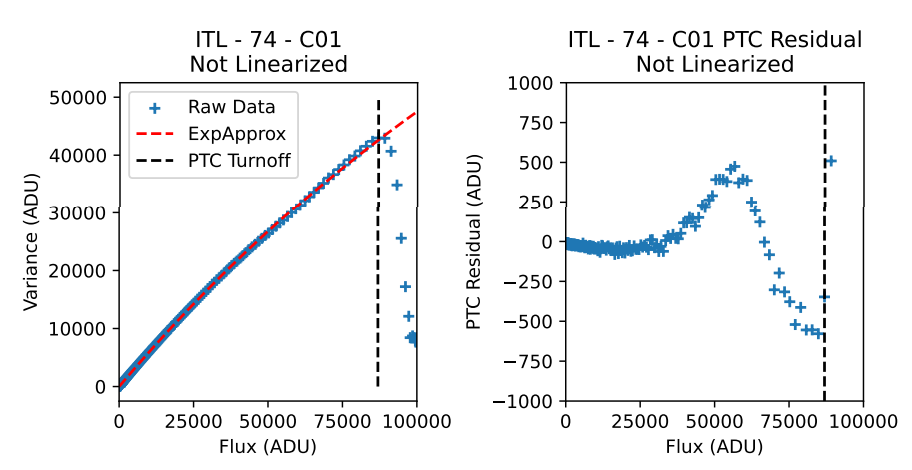
\includegraphics[width=0.75\textwidth]{Plots/Linearizer1.PNG}
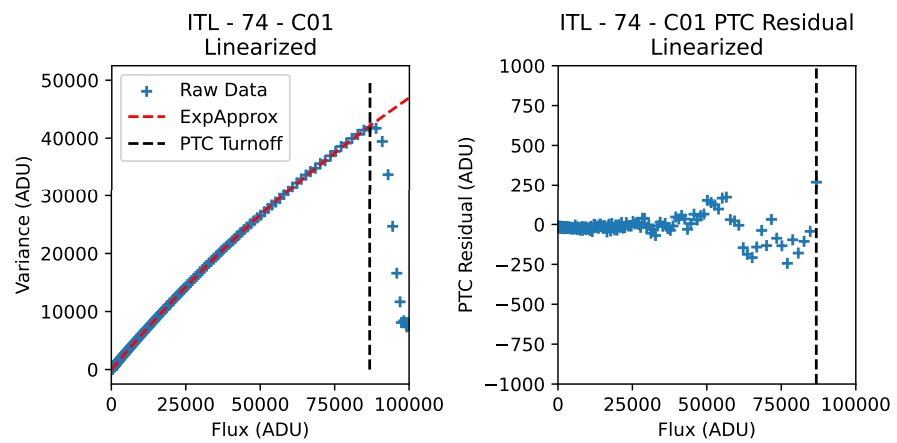
\includegraphics[width=0.75\textwidth]{Plots/Linearizer2.PNG}
\caption{\textit{Top: Non-linearized data. Bottom: Linearized data with 10 Spline knots (default setting).}}
\label{Linearizer1}
\end{center}
\end{figure}

\noindent Figure \ref{Linearizer2} shows the \textbf{linearization plots obtained with 11 Spline knots} for the same detector. Here we see in the top row the same plots we generated for fig. \ref{Linearizer1} but also in the bottom row we plot the knot distribution and the fit residual for the two iterations of the fit that the linearizer runs.\\

\begin{figure}[H]
\begin{center} 
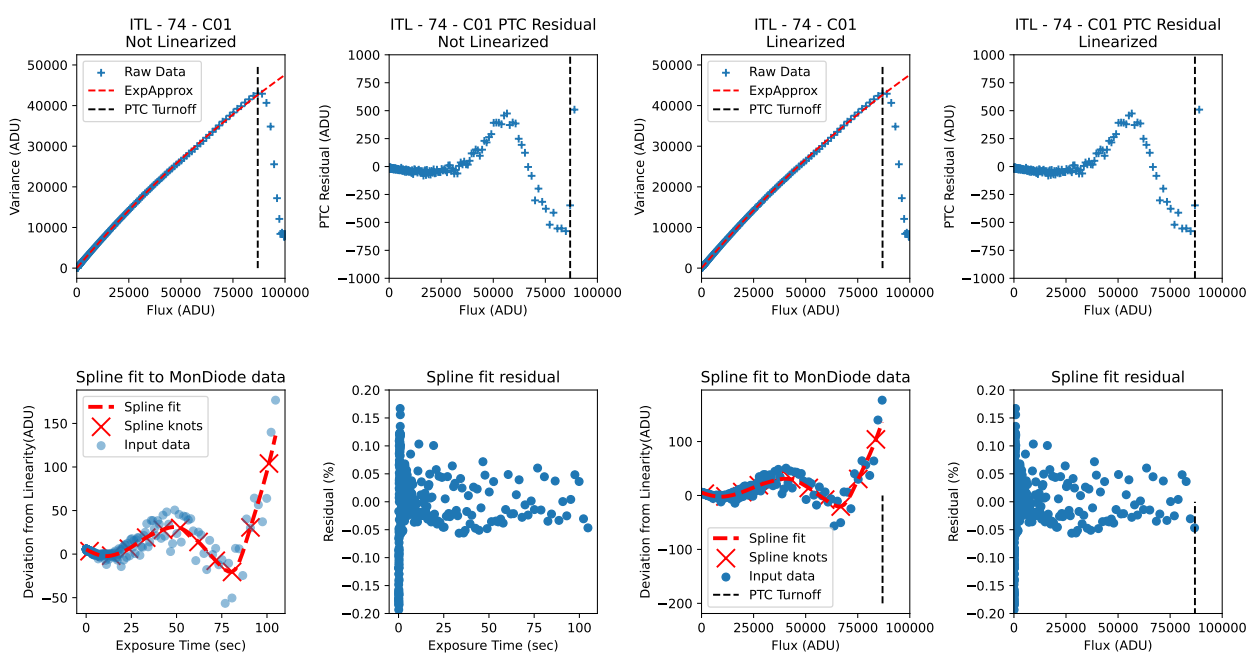
\includegraphics[scale=0.6]{Plots/linearizerSpline11knots.PNG}
\caption{\textit{Linearizer ran using 11 Spline knots. From top to bottom and from left to right we see the plots for: Non-linearized PTC, non-linearized PTC residuals from fit, linearized PTC, linearized PTC residuals from fit, spline knots used with the obtained deviation on the first fit, residual from first spline fit, spline knots used with the obtained deviation on the second fit, and residual from second spline fit. }}
\label{Linearizer2}
\end{center}
\end{figure}

\noindent In figure \ref{Linearizer3} we show a \textbf{comparison of the linearization with different number of Spline knots}. We notice how the same detector gets different PTC residuals from fitting splines of different number of knots. By inspecting the scattered points we see that 12 knots seems to give the best result, but we analyze this in further detail in section \ref{results}.\\

\begin{figure}[H]
\begin{center} 
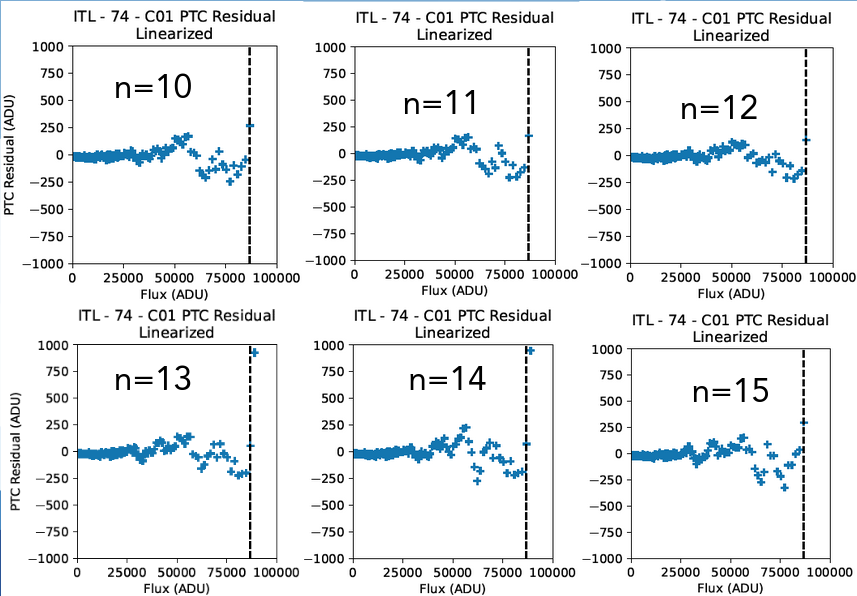
\includegraphics[width=0.7\textwidth]{Plots/LinearizersKnots_ITL74.png}
\caption{\textit{Deviation from linearity using different amount of knots.}}
\label{Linearizer3}
\end{center}
\end{figure}

\subsection{Changing the knot distribution}

\noindent A final test we ran was trying to fit the PTC using a non-uniform distribution of the Spline knots. With the help of Dr. Lage we ran the linearizer so that it used \textbf{10 evenly-spaced knots and around the 50000 ADU bump it added 5 extra knots between the others}. Figure \ref{Linearizer4} shows the results obtained and figures \ref{LinAmps1} and \ref{LinAmps2} show the deviation from linearity for all 16 amplifiers for 4 different detectors.

\begin{figure}[H]
\begin{center} 
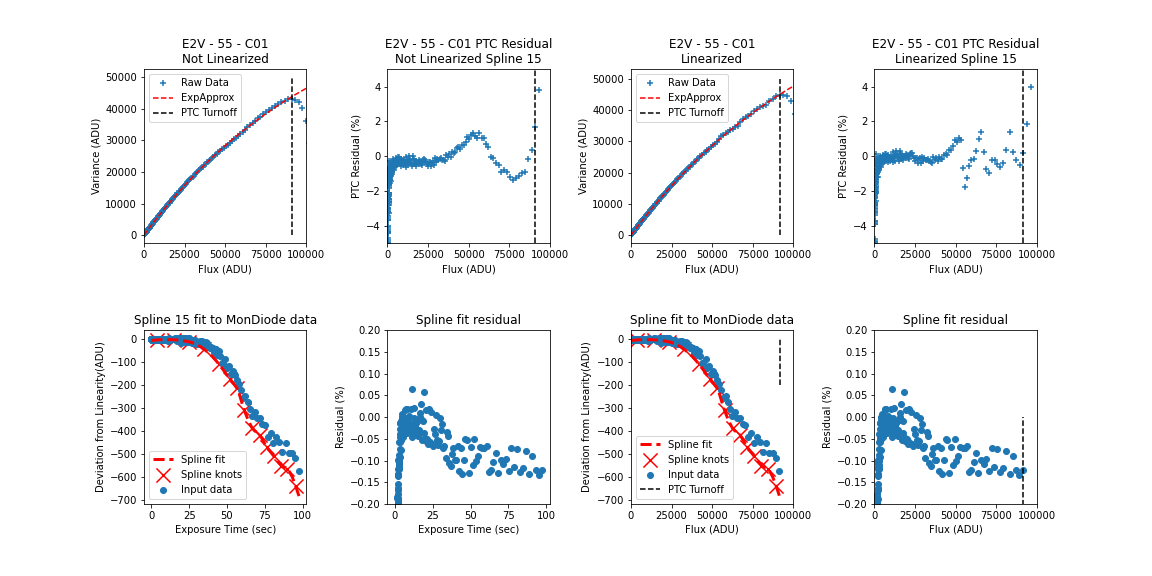
\includegraphics[scale=0.4]{Plots/E2V_55_C01_SplineNEStest.png}
\caption{\textit{Linearized PTC data for 10 equally spaced knots and 5 extra knots around the 50000 ADU bump.}}
\label{Linearizer4}
\end{center}
\end{figure}

\begin{figure}[H]
\begin{center} 
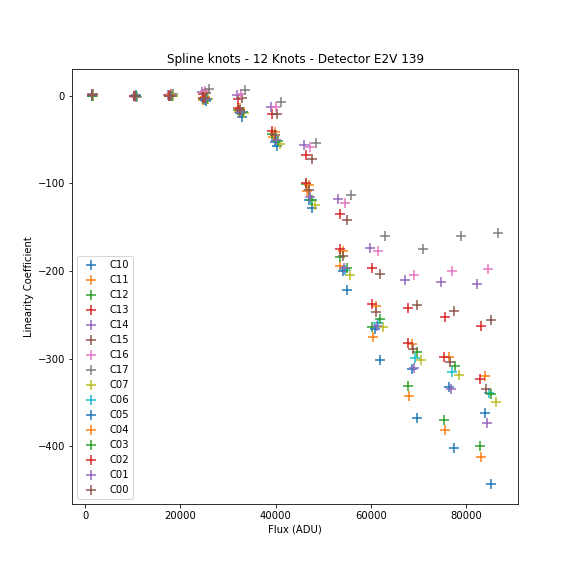
\includegraphics[scale=0.4]{Plots/Spline_Knots_E2V_Det139_15Aug22 (1).png}
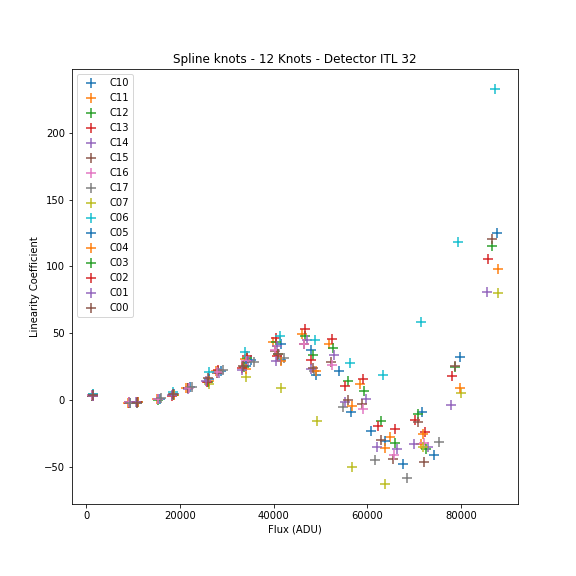
\includegraphics[scale=0.4]{Plots/Spline_Knots_ITL_Det32_15Aug22.png}
\caption{\textit{Deviation from linearity for the 16 amplifiers of detectors E2V 139 and ITL 32.}}
\label{LinAmps1}
\end{center}
\end{figure}

\begin{figure}[H]
\begin{center} 
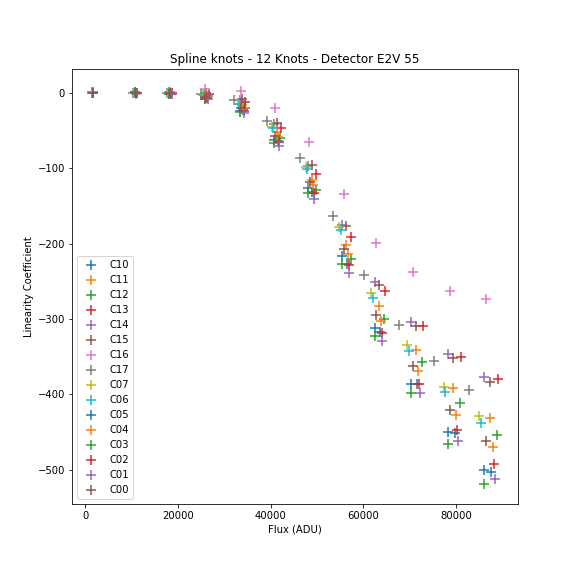
\includegraphics[scale=0.4]{Plots/Spline_Knots_E2V_Det55_29Jul22(1).png}
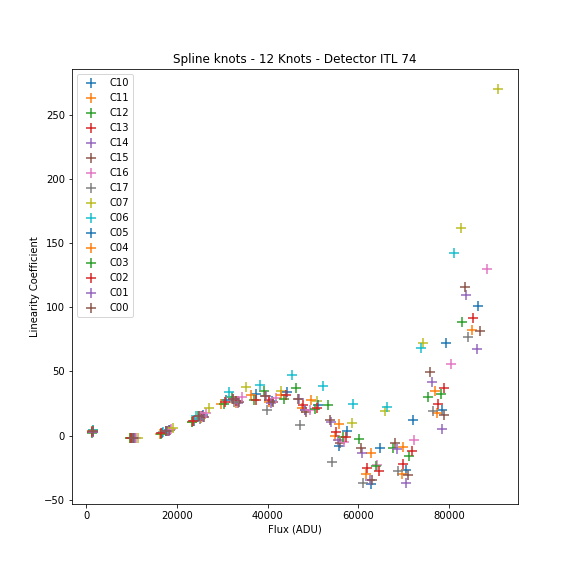
\includegraphics[scale=0.4]{Plots/Spline_Knots_ITL_Det74_29Jul22(1).png}
\caption{\textit{Deviation from linearity for the 16 amplifiers of detectors E2V 55 and ITL 74.}}
\label{LinAmps2}
\end{center}
\end{figure}

\subsection{Results and Conclusions}\label{results}

\noindent If we determine the average residual of the deviation from linearity in each case (no linearization, several spline knots with even spacing, and not evenly spaced knots) we can make plots like the ones shown in figures \ref{avgdeviation1} and \ref{avgdeviation2} in which we see how 12 Spline knots seems to be the right configuration for best linearization in both E2V and ITL detectors. Although we see that the difference between the 12-knot case and the others is not very significant, and mainly we can conclude that just \textbf{applying the linearizer with any of this configurations is much better than not linearizing at all}.\\

\begin{figure}[H]
\begin{center} 
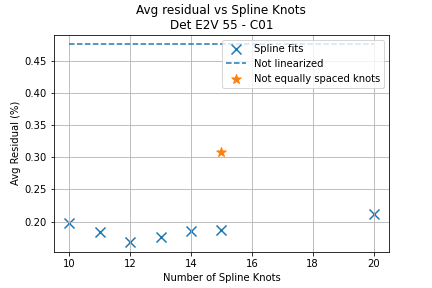
\includegraphics[scale=0.8]{Plots/AvgResvsKnots_55.png}
\caption{\textit{Average deviation for different fit types for detector E2V 55.}}
\label{avgdeviation1}
\end{center}
\end{figure}

\begin{figure}[H]
\begin{center} 
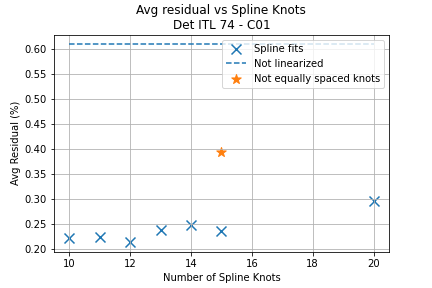
\includegraphics[scale=0.8]{Plots/AvgResvsKnots_74.png}
\caption{\textit{Average deviation for different fit types for detector ITL 74.}}
\label{avgdeviation2}
\end{center}
\end{figure}

\noindent We also note that the way we ran the linearizer with not-evenly-spaced knots resulted in overfitting and seems to have affected the quality of the linearization, we suggest this approach to be tested using maybe \textbf{more sofisticated algorithms that can optimize the position of the knots} to get below the 0.01\% deviation mark. One possibility would be to explore algorithms like LOESS\footnote{LOESS \url{https://towardsdatascience.com/loess-373d43b03564}} that use weight functions to smooth data with noise and get better fits. \\

\noindent During the presentation of this results to the DESC-SAWG meeting of the Rubin Observatory scientific team, Dr. Dan Weatherill pointed out an open problem about the fit residual plots (see fig. \ref{Linearizer2}) where indifferent laboratories, using different detectors \textbf{a bimodal behavior has been observed consistently} and is still not very well understood. This could be another interesting topic or future research in linearity for the LSSTCam.\\